\normalfalse \difficiletrue \tdifficilefalse
\correctiontrue

%\UPSTIidClasse{11} % 11 sup, 12 spé
%\newcommand{\UPSTIidClasse}{12}

\exer{Pompe à pistons radiaux  $\star\star$ \label{CIN:01:B2:12:11}}
\setcounter{question}{0}\marginnote{\xpComp{CIN}{01}}%\UPSTIcompetence{B2-12}
\index{Compétence B2-12}\index{Compétence CIN-01}
\index{Pompe à pistons radiaux}
\index{Arbre à cames}
\ifcorrection
\else
\marginnote{\textbf{Pas de corrigé pour cet exercice.}}
\fi

\ifprof
\else
Soit le mécanisme suivant. On a $\vect{AB}=e\vect{i_1}$ et $\vect{BI}=R\vect{j_0}$. De plus, 
$e=\SI{10}{mm}$ et $R=\SI{20}{mm}$. Le contact entre \textbf{1} et \textbf{2} en $B$ est maintenu en permanence par un ressort suffisamment raide (non représenté) positionné entre \textbf{0} et \textbf{2}. 
\begin{marginfigure}
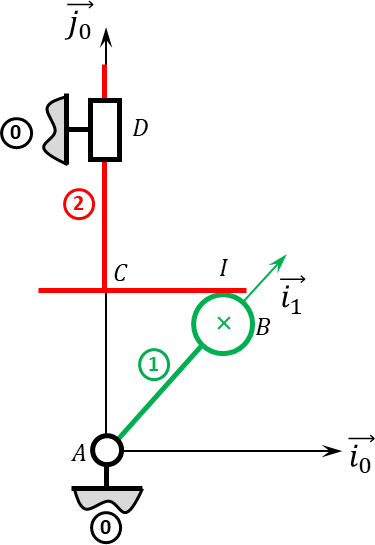
\includegraphics[width=\linewidth]{11_01}
\end{marginfigure}
\fi

\question{Tracer le graphe des liaisons.}
\ifprof
\begin{marginfigure}
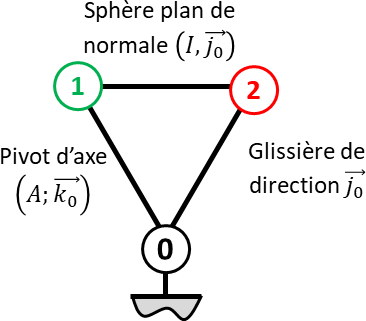
\includegraphics[width=4cm]{11_01_cor}
\end{marginfigure}
\else
\fi

\question{Retracer le schéma cinématique pour $\theta(t)=0 \,\text{rad}$.}
\ifprof
\else
\fi

\question{Retracer le schéma cinématique pour $\theta(t)=\dfrac{\pi}{2}\,\text{rad}$.}
\ifprof
\else
\fi

\question{Retracer le schéma cinématique pour $\theta(t)=-\dfrac{\pi}{2}\,\text{rad}$.}
\ifprof
\begin{marginfigure}
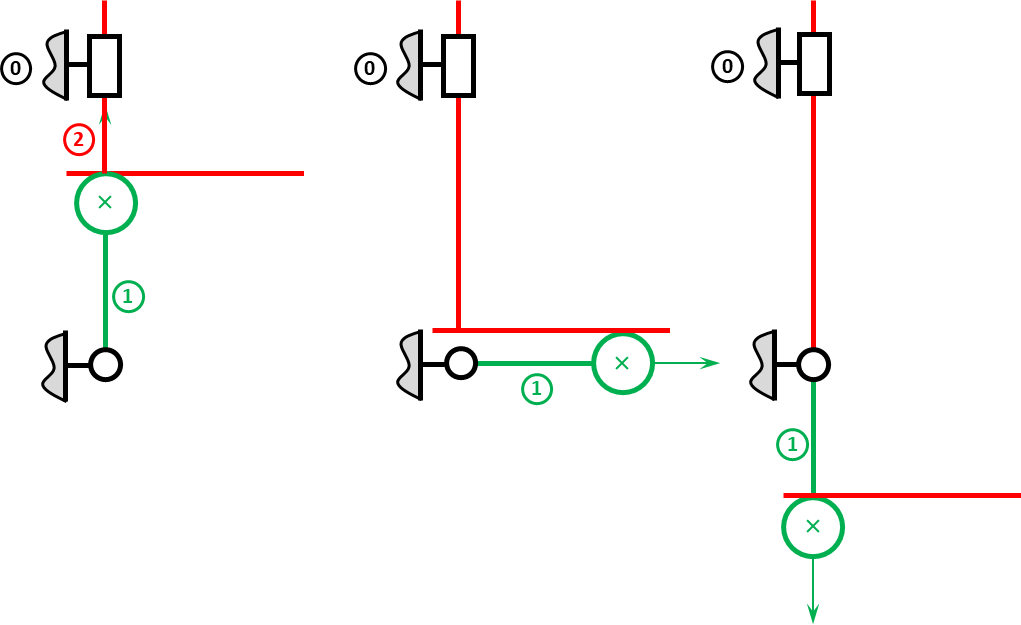
\includegraphics[width=8cm]{11_02_cor}
\end{marginfigure}
\else
\fi


\question{En déduire la course de la pièce \textbf{2}.}
\ifprof
La course est de 
\else
\fi



\ifprof
\else

\marginnote{Corrigé  voir \ref{CIN:01:B2:12:11}.}

\fi